A présent, nous allons replacer les visualisations que nous avons produites dans le contexte des humanités numériques actuelles.

Nous pouvons considérer qu'elles sont innovantes dans la mesure où l'utilisation de réseaux pour représenter les similarités entre différentes images reste encore rare. En effet, des projets comme Visual Contagion, iArt et ONiT Explorer favorisent encore largement la mosaïque malgré quelques tentatives de visualisation sous forme de carte chronologique ou de \textit{clusters}. 

Néanmoins, nous pouvons noter l'initiative récente que nous avons cité précédemment concernant l'étude des motifs similaires sur des tuiles chinoises\footcite{yuEmbodiedHeritageIntegrating2025a}. Les membres de l'équipe de recherche ont pour ambition de réaliser une visualisation en réseaux. Bien que ce projet suive une démarche comparable à la nôtre, il la dépasse en proposant une visualisation en réseaux tridimensionnelle associée à une frise chronologique. Leur prototype est composé de nœuds représentant les différentes tuiles relevées. Elles sont placées de manière horizontale à côté d'une chronologie en fonction de la période de leur création. Leur couleur diffère en fonction du type de motif qu'elles possèdent. Ils sont reliés entre eux par des liens semi-transparents dont la couleur indique leur type de motif. Ainsi, il est possible de conclure que l'époque des dynasties Qin et Han constitue l'apogée du développement de tuiles car nous observons une grande diversité de motifs. L'aspect tridimensionnel de la visualisation en réseaux améliore l'expérience de l'utilisateur qui peut alors la manipuler plus facilement pour observer les différents liens entre les nœuds\footcite{yuEmbodiedHeritageIntegrating2025a}. 

\begin{figure}[H]
	\centering
	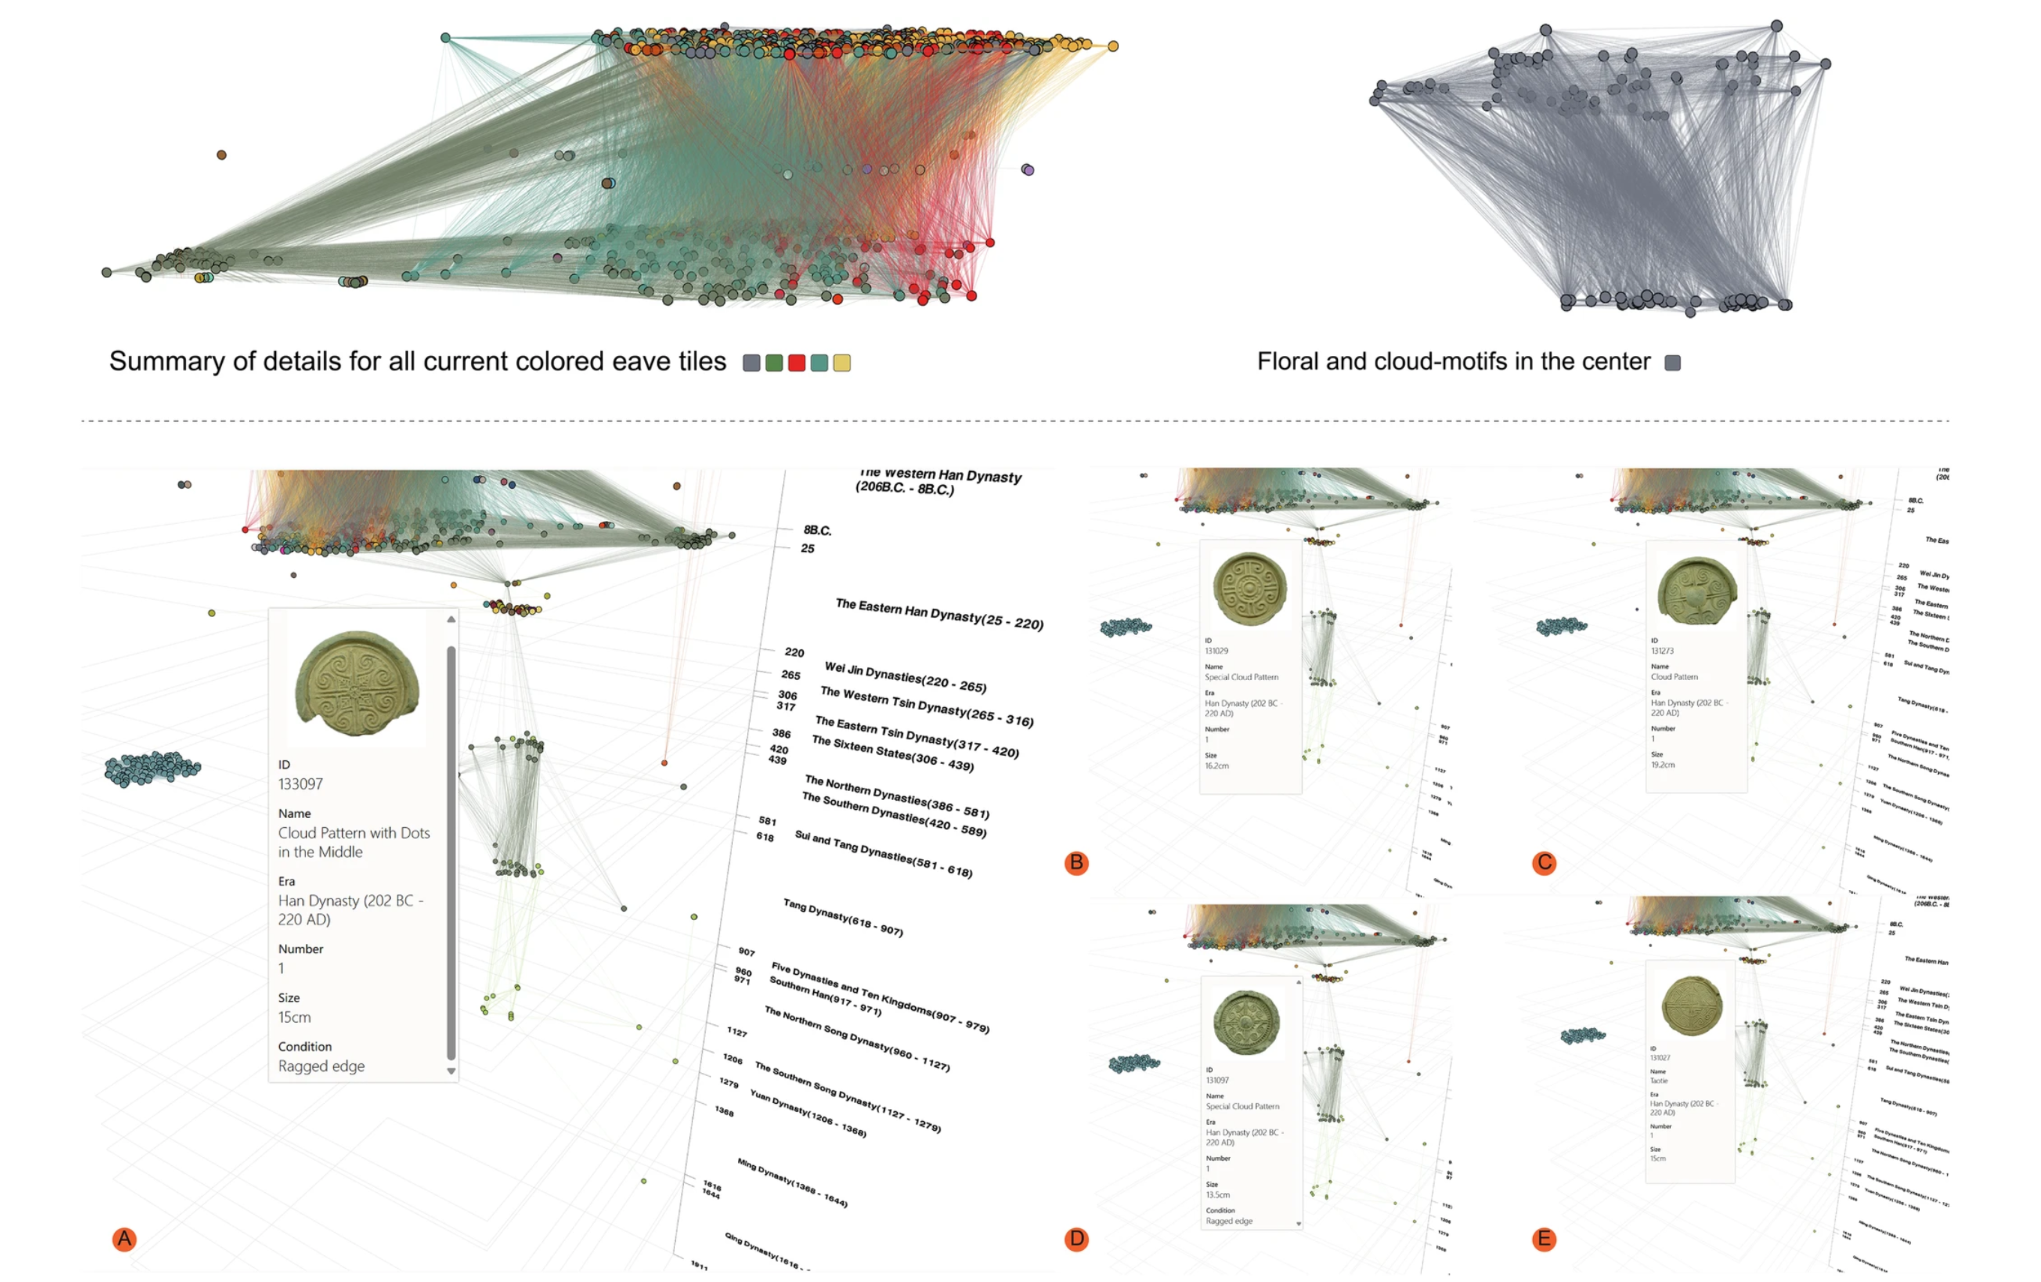
\includegraphics[width=1\textwidth]{images/prototype_visualisation_tuiles.png}
	\caption{Prototype de la visualisation tridimensionnelle extraite de l'article cité ci-dessus\footcite{yuEmbodiedHeritageIntegrating2025a}}
	\label{fig:prototypeprojettuiles}
\end{figure}

Pour améliorer la visualisation en réseaux que nous avons réalisé, nous pouvons envisager d'ajouter une frise chronologique pour montrer la diffusion des \textit{regions} similaires dans le temps. La modélisation 3D pourrait également faciliter la manipulation des différents éléments qui la composent. \\

